% Created 2023-03-17 Fri 14:36
% Intended LaTeX compiler: pdflatex
\documentclass[11pt]{article}
\usepackage[utf8]{inputenc}
\usepackage[T1]{fontenc}
\usepackage{graphicx}
\usepackage{longtable}
\usepackage{wrapfig}
\usepackage{rotating}
\usepackage[normalem]{ulem}
\usepackage{amsmath}
\usepackage{amssymb}
\usepackage{capt-of}
\usepackage{hyperref}
\usepackage{minted}
\usepackage[T2A]{fontenc}
\usepackage{parskip}
\usepackage[margin=0.5in]{geometry}
\usepackage{enumerate}
\usepackage{nopageno}
\author{megabluejay}
\date{}
\title{}
\hypersetup{
 pdfauthor={megabluejay},
 pdftitle={},
 pdfkeywords={},
 pdfsubject={},
 pdfcreator={Emacs 28.2 (Org mode 9.6.1)}, 
 pdflang={English}}
\begin{document}

\begin{center}
\textbf{Лабораторная 4}

Моисеев M33001, Муров M33011
\end{center}

\section*{Результаты}
\label{sec:org8fd4dfd}

\subsection*{a, c}
\label{sec:org3001743}

\begin{verbatim}
kernel='linear', nu=0.25
  accuracy=0.4956
  precision=0.1587719298245614
  recall=0.3747412008281574
  f1=0.2230437461491066

kernel='poly', nu=0.25
  accuracy=0.4992
  precision=0.27527761542957335
  recall=0.9751552795031055
  f1=0.4293527803099362

kernel='rbf', nu=0.25
  accuracy=0.984
  precision=1.0
  recall=0.917184265010352
  f1=0.9568034557235421

kernel='sigmoid', nu=0.25
  accuracy=0.4196
  precision=0.24896265560165975
  recall=0.9937888198757764
  f1=0.3981750311074243

kernel='rbf', nu=0.05
  accuracy=0.9972
  precision=0.9877049180327869
  recall=0.9979296066252588
  f1=0.9927909371781668

kernel='rbf', nu=0.2
  accuracy=0.9884
  precision=1.0
  recall=0.9399585921325052
  f1=0.9690501600853789

kernel='rbf', nu=0.3
  accuracy=0.9764
  precision=1.0
  recall=0.8778467908902692
  f1=0.9349503858875413
\end{verbatim}

\subsection*{графики}
\label{sec:org40b2fdb}

\subsubsection*{linear}
\label{sec:org2158bf1}

\begin{center}
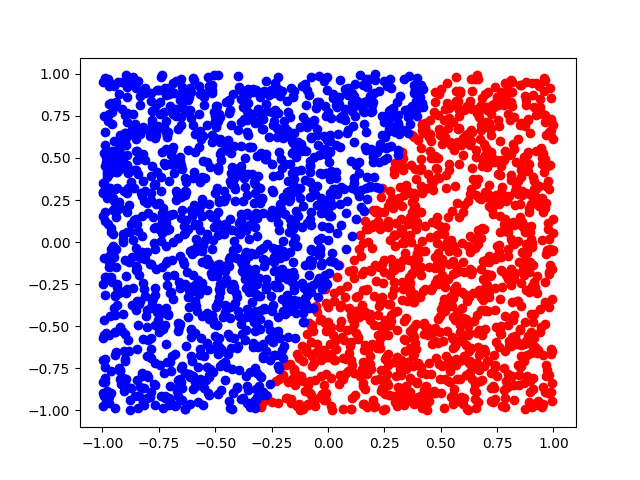
\includegraphics[scale=0.7]{./res/ac_points_linear_0.25.png}
\end{center}

\begin{center}
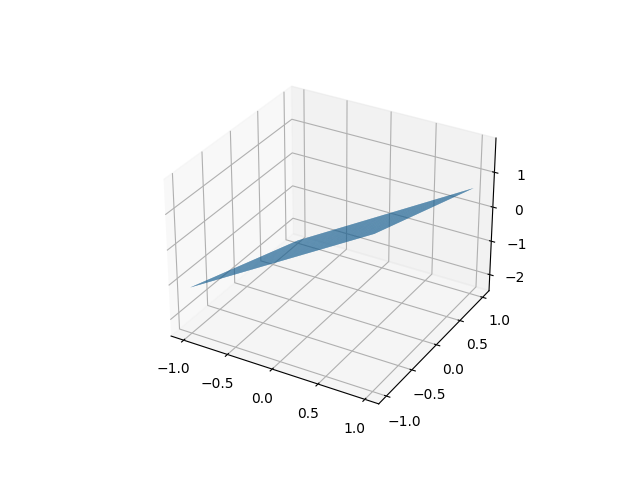
\includegraphics[scale=0.7]{./res/ac_surface_linear_0.25.png}
\end{center}

\subsubsection*{poly}
\label{sec:org12d4751}

\begin{center}
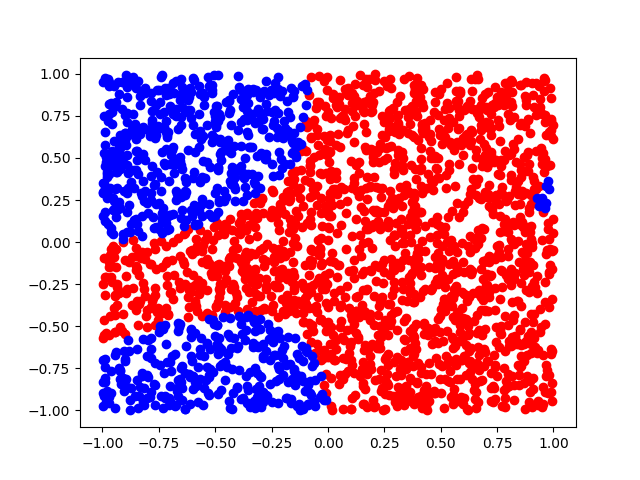
\includegraphics[scale=0.7]{./res/ac_points_poly_0.25.png}
\end{center}

\begin{center}
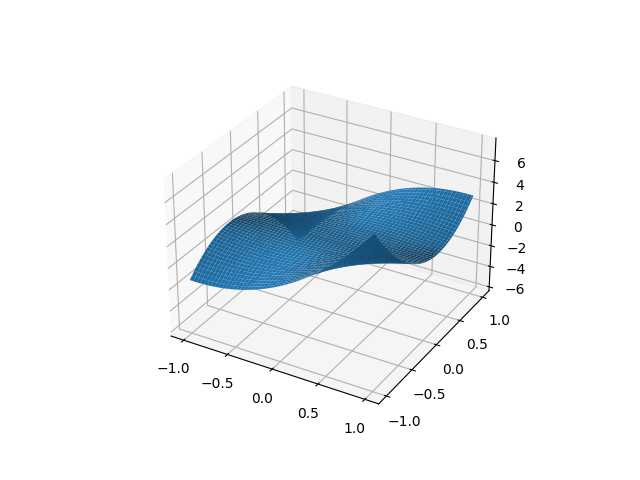
\includegraphics[scale=0.7]{./res/ac_surface_poly_0.25.png}
\end{center}

\subsubsection*{sigmoid}
\label{sec:orga0f27a3}

\begin{center}
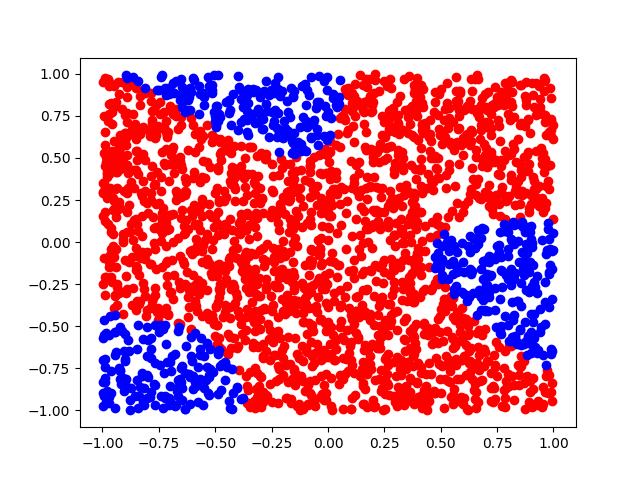
\includegraphics[scale=0.7]{./res/ac_points_sigmoid_0.25.png}
\end{center}

\begin{center}
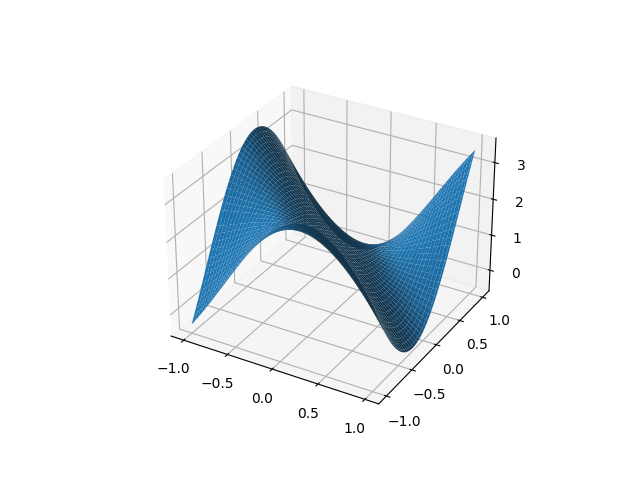
\includegraphics[scale=0.7]{./res/ac_surface_sigmoid_0.25.png}
\end{center}

\subsubsection*{rbf 0.25}
\label{sec:org85a4f2d}

\begin{center}
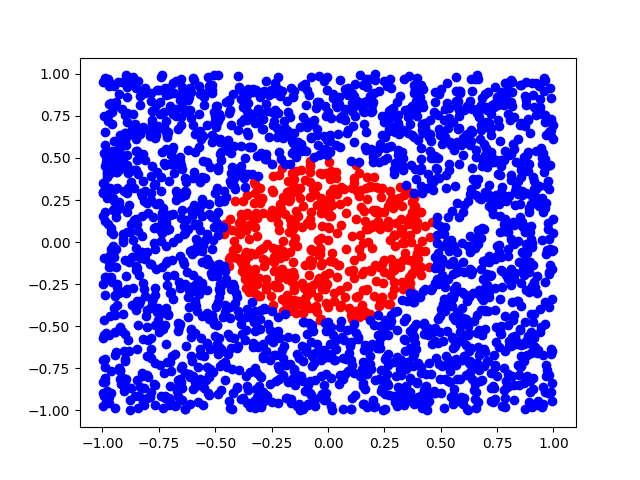
\includegraphics[scale=0.7]{./res/ac_points_rbf_0.25.png}
\end{center}

\begin{center}
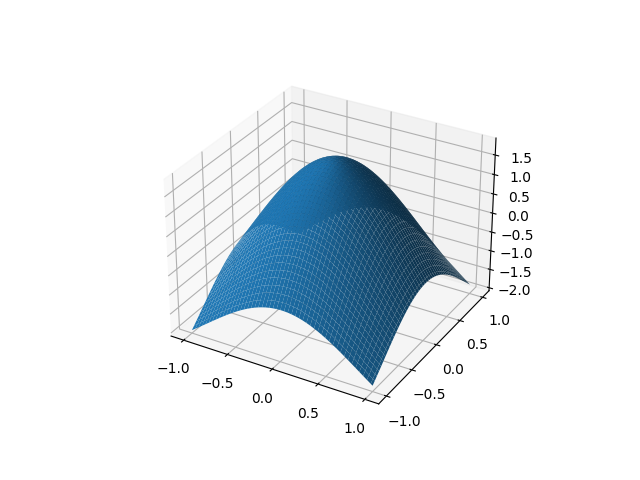
\includegraphics[scale=0.7]{./res/ac_surface_rbf_0.25.png}
\end{center}

\subsubsection*{rbf 0.05}
\label{sec:org2046337}

\begin{center}
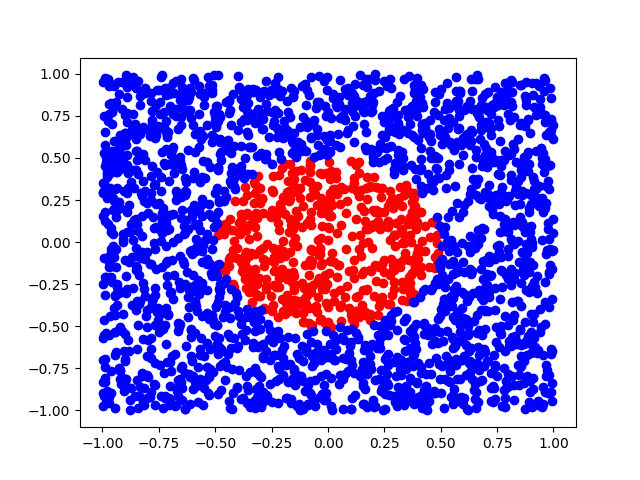
\includegraphics[scale=0.7]{./res/ac_points_rbf_0.05.png}
\end{center}

\begin{center}
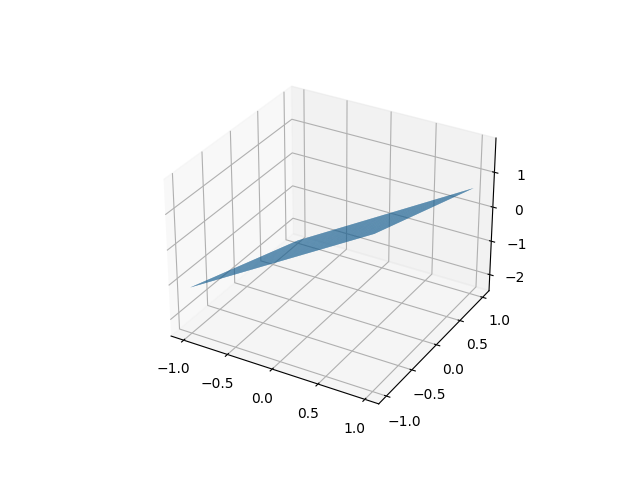
\includegraphics[scale=0.7]{./res/ac_surface_linear_0.25.png}
\end{center}

\subsubsection*{rbf 0.2}
\label{sec:org5c4c3f8}

\begin{center}
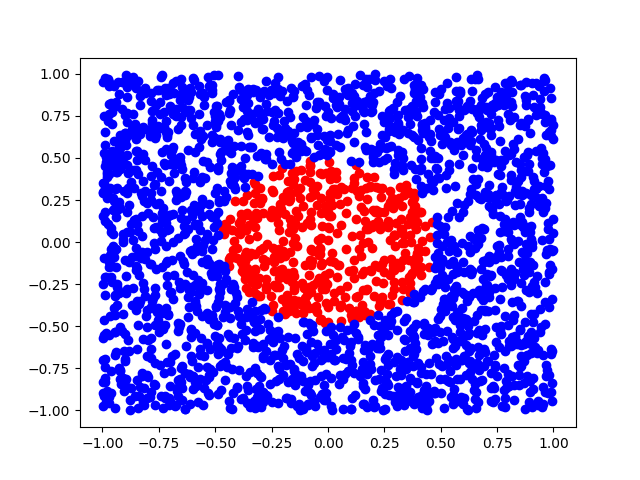
\includegraphics[scale=0.7]{./res/ac_points_rbf_0.2.png}
\end{center}

\begin{center}
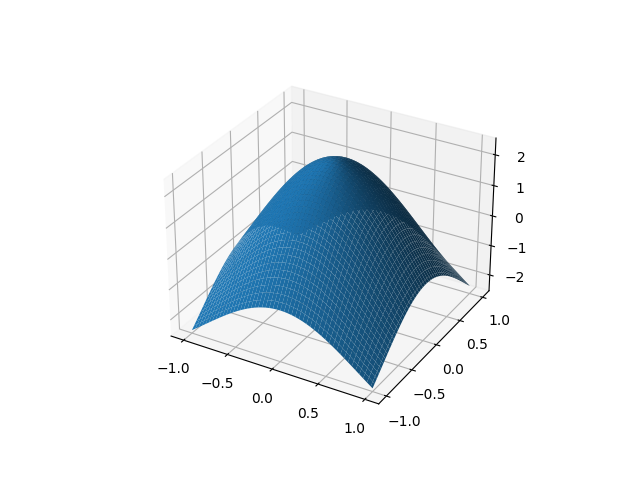
\includegraphics[scale=0.7]{./res/ac_surface_rbf_0.2.png}
\end{center}

\subsubsection*{rbf 0.3}
\label{sec:org998b7cb}

\begin{center}
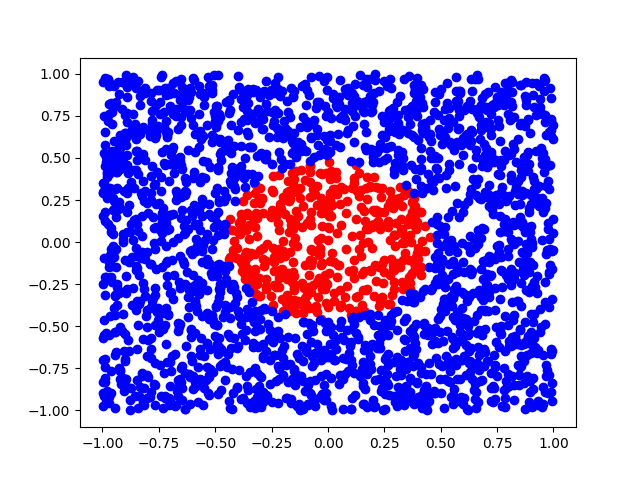
\includegraphics[scale=0.7]{./res/ac_points_rbf_0.3.png}
\end{center}

\begin{center}
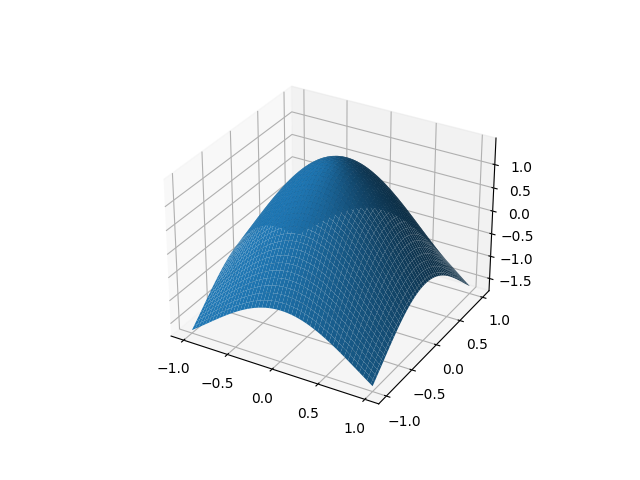
\includegraphics[scale=0.7]{./res/ac_surface_rbf_0.3.png}
\end{center}

\subsubsection*{accuracy}
\label{sec:org14b0499}

\begin{center}
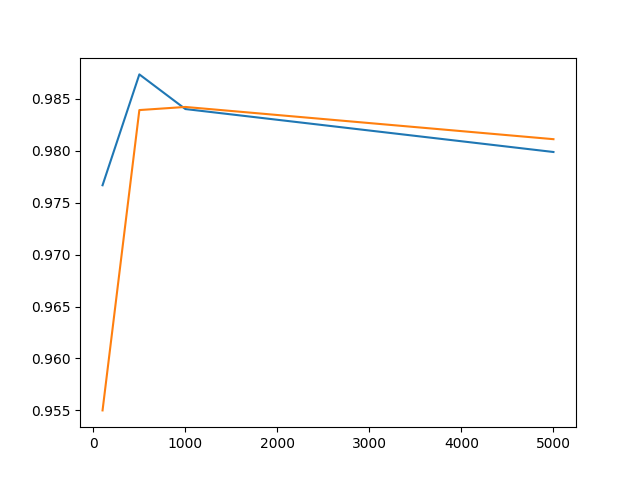
\includegraphics[scale=0.7]{./res/b_accuracy.png}
\end{center}

\subsubsection*{precision}
\label{sec:orgcb88ff2}

\begin{center}
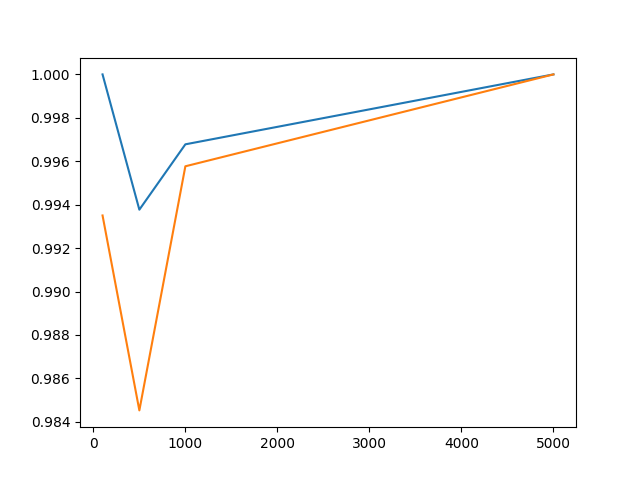
\includegraphics[scale=0.7]{./res/b_precision.png}
\end{center}

\subsubsection*{recall}
\label{sec:org1dde518}

\begin{center}
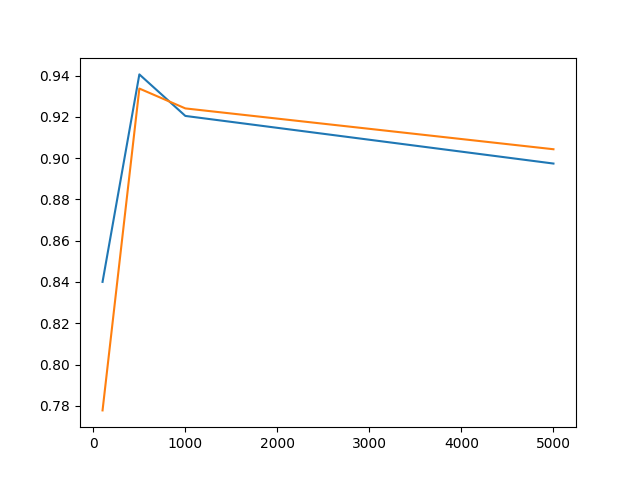
\includegraphics[scale=0.7]{./res/b_recall.png}
\end{center}

\subsubsection*{f1}
\label{sec:org52f3da3}

\begin{center}
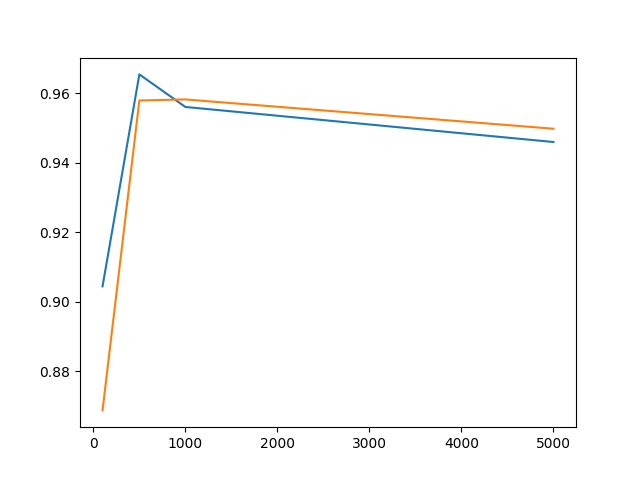
\includegraphics[scale=0.7]{./res/b_f1.png}
\end{center}

\section*{Код}
\label{sec:org18f4c88}

\subsection*{1}
\label{sec:org89cd141}

\begin{minted}[]{python}
import numpy as np

rng = np.random.default_rng()


def generate(n):
    x = rng.uniform(-1, 1, (n, 2))
    y = x[:, 0] ** 2 + x[:, 1] ** 2 <= 0.25
    return x, y
\end{minted}

\subsection*{2}
\label{sec:orgfacef09}

\begin{minted}[]{python}
import numpy as np
from sorcery import dict_of


def accuracy(y, y_pred):
    return np.count_nonzero(y == y_pred) / y.size


def precision(y, y_pred):
    return np.count_nonzero(y_pred[y]) / np.count_nonzero(y_pred)


def recall(y, y_pred):
    return np.count_nonzero(y_pred[y]) / np.count_nonzero(y)


def f1(y, y_pred):
    return 2 * np.count_nonzero(y_pred[y]) / (np.count_nonzero(y_pred) + np.count_nonzero(y))


metrics = dict_of(accuracy, precision, recall, f1)
\end{minted}

\subsection*{3}
\label{sec:org9ff7f1e}

\begin{minted}[]{python}
import sys
from pathlib import Path

import numpy as np
import matplotlib.pyplot as plt
from sklearn.model_selection import learning_curve, train_test_split
from sklearn.metrics import make_scorer
from sklearn.preprocessing import StandardScaler
from sklearn.svm import NuSVC

from .gen import generate
from .metrics import metrics

res_dir = str(Path(__file__).parent.resolve() / "res")
sys.stdout = open(f"{res_dir}/text", "w")

Xog, y = generate(10_000)
X = StandardScaler().fit_transform(Xog)
Xog_train, Xog_test, X_train, X_test, y_train, y_test = train_test_split(Xog, X, y)

xx, yy = np.meshgrid(np.linspace(-1, 1, 100), np.linspace(-1, 1, 100))


def do_ac(kernel="rbf", nu=0.25):
    svc = NuSVC(kernel=kernel, nu=nu)
    svc.fit(X_train, y_train)
    y_pred = svc.predict(X_test)

    print(f"{kernel=}, {nu=}")
    for name, metric in metrics.items():
        print(f"  {name}={metric(y_test, y_pred)}")
    print()

    plt.plot(Xog_test[y_pred, 0], Xog_test[y_pred, 1], "ro")
    plt.plot(Xog_test[~y_pred, 0], Xog_test[~y_pred, 1], "bo")
    plt.savefig(f"{res_dir}/ac_points_{kernel}_{nu}.png")
    plt.clf()

    fig, ax = plt.subplots(subplot_kw={"projection": "3d"})
    z = svc.decision_function(np.c_[xx.ravel(), yy.ravel()]).reshape(xx.shape)
    ax.plot_surface(xx, yy, z)
    plt.savefig(f"{res_dir}/ac_surface_{kernel}_{nu}.png")
    plt.clf()


for kernel in ["linear", "poly", "rbf", "sigmoid"]:
    do_ac(kernel=kernel)
for nu in [0.05, 0.2, 0.3]:
    do_ac(nu=nu)

for name, metric in metrics.items():
    train_sizes, train_scores, test_scores = learning_curve(
        NuSVC(kernel="rbf", nu=0.25),
        X,
        y,
        cv=3,
        scoring=make_scorer(metric),
        train_sizes=[10, 50, 100, 500, 1000, 5000],
    )
    plt.plot(train_sizes, np.mean(train_scores, axis=1))
    plt.plot(train_sizes, np.mean(test_scores, axis=1))
    plt.savefig(f"{res_dir}/b_{name}.png")
    plt.clf()

sys.stdout.close()
\end{minted}
\end{document}